\section{System Perspective}
\subsection{Design and architecture}

\subsubsection{Design}
The first step of taking over the Minitwit system required a refactoring to a different technology stack. 
As a group we chose a full .NET stack because every member of the felt comfortable and experienced with both backend and front-end development using C\#. The group wanted to focus on learning the new tools and working in a “DevOps” manner, and we recognized that experience would simplify the process.

For the front-end we went with Blazor-WASM and for our backend we decided used a traditional ASP.NET API. When refactoring the Flask application we did it in small steps making sure to preserve the functionality and style of the original.

\subsubsection{Deployment architecture}
The overall architecture of our deployed MiniTwit service can be seen on figure \ref{fig:deploy-meta}. As seen on the figure all our nodes in the system are run as virtual machines (or droplets) on DigitalOcean, we even decided to self-host the database to experience the challenges that go along with doing so.
\\
As scaling/load balancing was one of the weekly tasks, we introduced it into the architecture in the form of a Docker swarm. More specifically, we deployed our simulation API to a Docker swarm with a total of three nodes, one manager and two workers. Our Docker swarm would replicate NetData globally, a tool we use for monitoring hardware, and only replicate our simulation API on a single node.
%\tobedeleted{why did we choose to only replicate our simAPI on a single node? Cost?}
When deciding on a scaling strategy, we also discussed the possibility of creating a swarm for our front-end. Ultimately, we decided to keep it a single node, since the cost of instantiating a swarm was too high compared to the amount of front-end users.

%\tobedeleted{Okay this sounds nice, but we don't actually monitor our front-end, LOL, maybe we should fix. Like how would we know how many people are using our frontend? Sussy}

To do monitoring and logging of the system, a \textit{utility node} was set up. The utility node would host tools like Grafana, Kibana, postgres, and be in charge of collecting the monitoring data through Prometheus. The utility node as such communicates with most other nodes in the system.

%Not sure what else there to say, that describes our architecture, me thinks

\begin{figure}
    \centering
    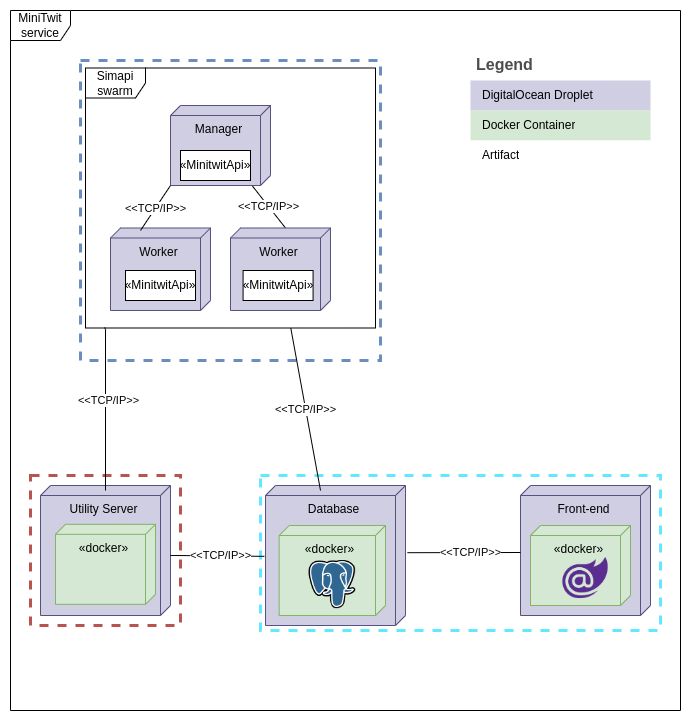
\includegraphics[scale=0.4]{images/Deployment-meta.png}
    \caption{UML Deployment Diagram—Shows the overall architecture of our deployed MiniTwit service. Dashed colored lines indicate different zooms of the architecture.  \hyperref[sec:dep_sim]{Simulator zoom}(\ref{sec:dep_sim}),
     \hyperref[sec:dep_front]{Front-end zoom}(\ref{sec:dep_front}), \hyperref[sec:dep_utility]{Utility zoom}(\ref{sec:dep_utility}).}
    \label{fig:deploy-meta}
\end{figure}

\subsubsection{Code architecture:}
Our system is fully contained in the .NET environment, that is our front-end, backend, and simulator API are all built using .NET. 
At compile-time every module/project depends on domain model which exists in our MiniTwit.Shared library, as can be seen on figure \ref{fig:module-digram}. 

\begin{figure}
    \centering
    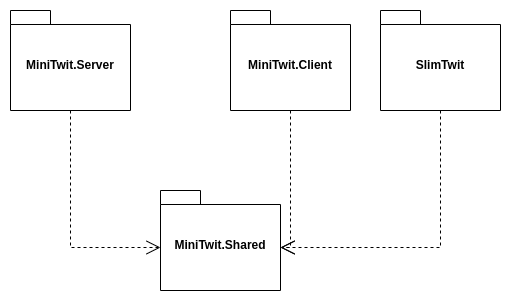
\includegraphics[scale=0.5]{images/ModuleDiagram.png}
    \caption{UML Module Diagram - shows the compile time dependencies within our own modules}
    \label{fig:module-digram}
\end{figure}


\subsection{The System's Dependencies}
\subsubsection{Nuget}
\begin{table}[H]
    \hspace*{-3cm}
    \centering
    \resizebox{1.5\textwidth}{!}{
        \begin{tabular}{|c|c|c|c|c|c|c|}
        \hline
        & Server.Test & e2e & SlimTwit & MiniTwit.Shared & MiniTwit.Client & MiniTwit.Server \\\hline
        Microsoft.EntityFrameworkCore.InMemory & x &  & x &  &  & x \\\hline
        Npgsql.EntityFrameworkCore.PostgreSQL &  &  & x &  &  & x \\\hline
        Microsoft.AspNetCore.Components.WebAssembly.Server &  &  &  &  &  & x \\\hline
        Microsoft.AspNetCore.Mvc.Testing & x &  &  &  &  & x \\\hline
        Microsoft.EntityFrameworkCore & x &  & x & x &  & x \\\hline
        Microsoft.EntityFrameworkCore.Design &  &  &  &  &  & x \\\hline
        Newtonsoft.Json &  &  &  & x & x & x \\\hline
        Serilog.AspNetCore & x &  & x &  &  & x \\\hline
        Serilog.Sinks.Console & x &  & x &  &  & x \\\hline
        Serilog.Sinks.Elasticsearch & x &  & x &  &  & x \\\hline
        SQLite  &  &  &  &  & x & x \\\hline
        Microsoft.AspNetCore.Components.WebAssembly.DevServer &  &  &  &  & x &  \\\hline
        Bogus &  &  &  & x &  &  \\\hline
        Microsoft.EntityFrameworkCore.Sqlite & x &  &  & x &  &  \\\hline
        Microsoft.AspNetCore.OpenApi &  &  & x &  &  &  \\\hline
        prometheus-net &  &  & x &  &  &  \\\hline
        prometheus-net.AspNetCore &  &  & x &  &  &  \\\hline
        Swashbuckle.AspNetCore &  &  & x &  &  &  \\\hline
        coverlet.collector & x & x &  &  &  &  \\\hline
        FluentAssertions & x & x &  &  &  &  \\\hline
        Microsoft.AspNetCore.TestHost & x &  &  &  &  &  \\\hline
        Microsoft.Data.Sqlite & x &  &  &  &  &  \\\hline
        Microsoft.NET.Test.Sdk & x & x &  &  &  &  \\\hline
        xunit & x &  &  &  &  &  \\\hline
        xunit.runner.visualstudio & x &  &  &  &  &  \\\hline
        Microsoft.Playwright.Nunit &  & x &  &  &  &  \\\hline
        NUnit &  & x &  &  &  &  \\\hline
        NUnit.Analyzers &  & x &  &  &  &  \\\hline
        NUnit3TestAdapter &  & x &  &  &  &  \\
        \hline
    \end{tabular}
    }
    \caption{The full list of all 29 Nuget dependencies in our system, and what dotnet projects they belong to.}
    \label{tab:dependencies}
\end{table}
\subsubsection{Tools \& Other Dependencies}
\begin{itemize}
    \item Docker for containerization \& Swarm
    \item DigitalOcean for hosting
    \item Terraform for infrastructure as code
    \item Prometheus for monitoring
    \item Grafana for visualizing data from Prometheus
    \item Dependabot for updating dependencies automatically
    \item SonarCloud as code review tool
    \item Serilog for logging
    \item Kibana for visualizing data from Serilog
    \item NetData For monitoring health of hardware
    \item Playwright / nUnit for E2E testing
    \item xUnit for unit testing
    \item \st{Vagrant for VM configuration}
\end{itemize}

\subsection{Important interactions of subsystems}
A very important interaction for service is the interaction with the database which both the front-end system and simulation API need to do. The interaction is similar for both systems, both systems use our \textit{TwitContext} to query and save entities in the database, this interaction can be seen on figure \ref{fig:componentsAndConnector}.

\begin{figure}[h]
    \centering
    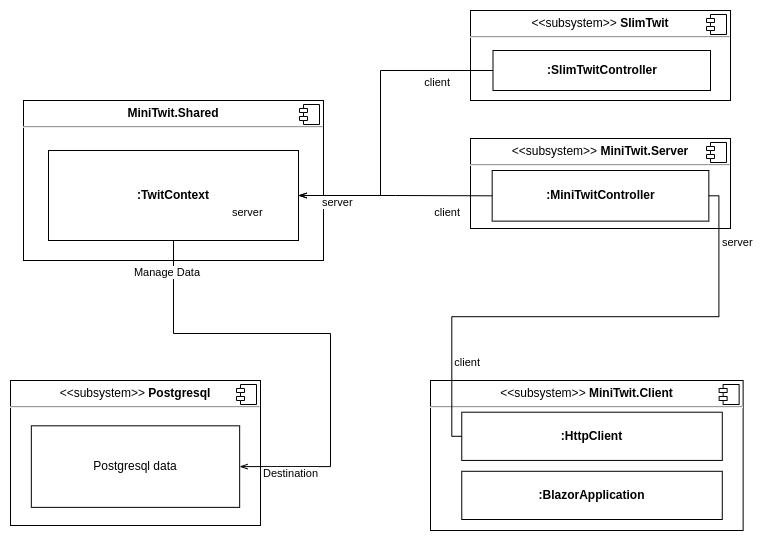
\includegraphics[width=\linewidth]{ComponentsAndConnector.png}
    \caption{Components and Connector diagram showing how our system reaches the database through EFCore}
    \label{fig:componentsAndConnector}
\end{figure}
\newpage

\subsection{The current state of our systems}
The system is fully containerized, meaning it is independent of the development and deployment environment. Similarly, the containerization allows deploying the system to a Docker swarm increasing availability.
To increase the reliability, the CI/CD pipeline now includes quality gates in the form of static code analysis and tests.
Since taking over the Minitwit system it has been refactored to a statically typed language and the system receives an \textit{A} in the maintainability category in the Sonarcloud static code report 
\footnote{ Sonarcloud report can be here: 
 \url{https://sonarcloud.io/summary/overall?id=bhviid_GroupJ_Dev_Ops23} } 
(which should be taken with a grain of salt, as there are still 15 code smells and at least two known bugs).
\\
For the current state, it is important to note that the database runs incredibly slow. Some often done SQL joins take upwards of seconds and regularly going beyond 10 seconds.
\\
\\
We would have liked to improve the system by:
\begin{itemize}
    \item Implementing the repository pattern for the database interaction to reduce the amount of duplicated logic for front-end and simulation API.
    \item Properly running end-to-end tests in the CI pipeline.
    \item Successfully creating indexes for the database.
    \item Making the front-end design more modern
    
\end{itemize}

\subsection{License}
We did not discuss licenses while the project was going on, but we would likely have gone with GPL 3.0 or Apache 2.0, as these are the more restrictive out of the ones that occur in our dependencies, and we want to keep it open source. We used a tool called choosealicense.com to reach this conclusion.
